\section{AFD Paridad en números binarios}
	\subsection{Descripción del problema}
	Diseñar y programar un autómata finito determinista que acepte el lenguaje:
	\[ L = \lbrace w \mid w \text{ tiene un número par de ceros y un numero par de unos} \rbrace \text{\cite{LIBRO}}\] 
	Es decir, los números binarios de entrada se generan de manera automática (cadena de longitud $n \mid 1\leq n \leq 1000$) o manual y después se imprime si es una cadena valida o no y en ambos casos imprimir su historia. Ademas, mostrar el siguiente diagrama.
	\begin{figure}[H]
		\begin{center}
			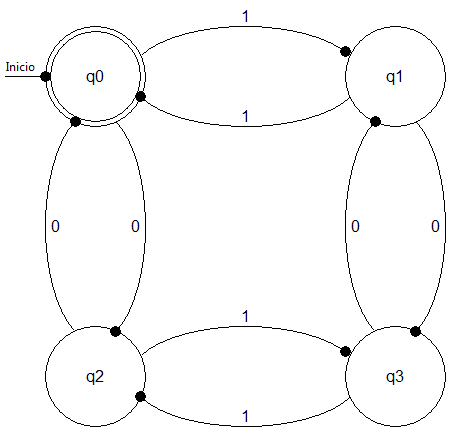
\includegraphics[width=7cm, height=7cm]{img/paridad.png}
			\caption{Diagrama de transiciones del autómata. \cite{LIBRO}}
			\label{fig:diagrama2}
		\end{center}
	\end{figure}
	\subsection{Código}
	El código fue realizado en Python 3.5.
	\\Archivo: main\_paridad.py
	\begin{lstlisting}[language=Python]
	#main_paridad.py
	# -*- coding: utf-8 -*-
	from __future__ import print_function
	from automata_paridad import ejecutar_automata
	from diagrama_paridad import Diagrama
	import random
	
	separador = '*' * 50
	def iniciar():
		continuar = True
		while continuar:
			opcion = imprimir_menu()
			if opcion == 1:
				ejecutar_manual()
			elif opcion == 2:
				ejecutar_random()
			elif opcion == 3:
				ver_diagrama()
			else:
				break
			print('\n', separador)
			opcion = input("Reintentar s/n: ")
			if opcion.lower() != 's':
				continuar = False
		
		print('Saliendo del programa...')
	
	def imprimir_menu():
		print('\n\n%sMenu%s' % (separador, separador))
		print("""
		1.- Entrada en consola (Manual)
		2.- Numero aleatorio (automatico)
		3.- Ver diagrama de transiciones
		4.- Salir
		""")
		try:
			opcion = int(input("Selecciona una opcion valida: "))
			return opcion
		except Exception as e:
			print('Error ', e)
			return 0
	
	def ejecutar_random():
		i = 0
		longitud_random = random.randint(1, 1000)
		numero_binario = ''
		while i < longitud_random:
			numero_binario += random.choice(['0', '1'])
			i += 1
		
		print("El numero aleatorio es: ", numero_binario)
		provar_paridad(numero_binario)
	
	def ejecutar_manual():
		numero_binario = input("Escribe un numero binario: ")
		provar_paridad(numero_binario)
	
	def provar_paridad(numero_binario):
		resultado = ejecutar_automata(numero_binario)
		print('\n')
		if resultado:
			print('El numero %s, es valido' % numero_binario)
		else:
			print('El numero: %s, no es valido' % numero_binario)
	
	def ver_diagrama():
		print('Mostrando diagrama del automata. Cierre la ventana para continuar')
		try:
			diagrama_paridad = Diagrama()
			diagrama_paridad.master.title('Diagrama del automata paridad')
			diagrama_paridad.mainloop()
		except Exception as e:
			print("Error", e)
	
	iniciar()
	\end{lstlisting}
	Archivo: automata\_paridad.py
	\begin{lstlisting}[language=Python]
	#automata_paridad.py
	def ejecutar_automata(cadena):
		estado = 0
		for simbolo in cadena:
			print('-> delta(q%s,%s)' % (estado, simbolo), end="\t")
			estado = automata(estado, simbolo)
			if estado == -1:
				break
		if estado == 0:
			print('-> delta(q%s, )' % estado, end="\t")
			return True
		return False
	
	def automata(estado, simbolo):
		if estado == 0:
			estado = estado_cero(simbolo)
		elif estado == 1:
			estado = estado_uno(simbolo)
		elif estado == 2:
			estado = estado_dos(simbolo)
		elif estado == 3:
			estado = estado_tres(simbolo)
		else:
			print('Simbolo extrano ', simbolo)
			return -1
		return estado
	
	def estado_cero(simbolo):
		if simbolo == '0':
			return 2
		elif simbolo == '1':
			return 1
		else:
			return -1
	
	def estado_uno(simbolo):
		if simbolo == '0':
			return 3
		elif simbolo == '1':
			return 0
		else:
			return -1
		
	def estado_dos(simbolo):
		if simbolo == '0':
			return 0
		elif simbolo == '1':
			return 3
		else:
			return -1
	
	def estado_tres(simbolo):
		if simbolo == '0':
			return 1
		elif simbolo == '1':
			return 2
		else:
			return -1
	\end{lstlisting}
	Archivo: diagrama\_paridad.py
	\begin{lstlisting}[language=Python]
	#diagrama_paridad.py
	# -*- coding: utf-8 -*-
	from __future__ import print_function
	import tkinter as tk
	
	class Diagrama(tk.Frame):
		def __init__(self, master=None):
			super().__init__(master, background='white')
			self.pack(fill=tk.BOTH, expand=tk.YES)
			self.canvas = tk.Canvas(self, bg='white')
			self.canvas.pack(fill=tk.BOTH, expand=1)
			self.dibujarDiagrama()
			self.centrarVentana()
		
		def dibujarDiagrama(self):
			self.dibujarFlecha([10, 100, 50, 100])
			self.dibujarCirculo([55, 55, 145, 145])
			for x in range(4):
				if x == 0:
					coordenadas = [50, 50, 150, 150]
					text_circulo = 'q%s' % x
					self.dibujarFlechaHorizontal(coordenadas[:])
					self.dibujarFlechaVertical(coordenadas[:])
				elif x == 1:
					coordenadas = [350, 50, 450, 150]
					text_circulo = 'q%s' % x
					self.dibujarFlechaVertical(coordenadas[:])
				elif x == 2:
					coordenadas = [50, 350, 150, 450]
					text_circulo = 'q%s' % x
					self.dibujarFlechaHorizontal(coordenadas[:])
				elif x == 3:
					coordenadas = [350, 350, 450, 450]
					text_circulo = 'q%s' % x
				
				else:
					print('Na')
				
				self.dibujarCirculo(coordenadas)
				self.canvas.create_text(coordenadas[0]+50, coordenadas[1]+50, font=('15'), text=text_circulo)
			
		def dibujarCirculo(self, arg):
			circulo = self.canvas.create_oval(arg)
		
		def dibujarFlechaHorizontal(self, coordenadas):
			coordenadas[0] += 85
			coordenadas[2] += 215
			x = ((coordenadas[2] - coordenadas[0])/2) + coordenadas[0]
			
			self.canvas.create_text(x, coordenadas[1]-10, font=('15'), text='1')
			self.canvas.create_text(x, coordenadas[3]-10, font=('15'), text='1')
			
			self.canvas.create_arc(coordenadas, start=25, extent=130, style='arc')
			self.canvas.create_arc(coordenadas, start=-25, extent=-130, style='arc')
			
			self.canvas.create_oval(coordenadas[2]-5-15, coordenadas[1]-5+25, coordenadas[2]+5-15, coordenadas[1]+5+25, fill = 'black')
			self.canvas.create_oval(coordenadas[0]-5+10, coordenadas[3]-5-30, coordenadas[0]+5+10, coordenadas[3]+5-30, fill = 'black')
		
		def dibujarFlechaVertical(self, coordenadas):
			coordenadas[1] += 85
			coordenadas[3] += 215
			
			y = ((coordenadas[3] - coordenadas[1])/2) + coordenadas[1]
			
			self.canvas.create_text(coordenadas[0]+10, y, font=('15'), text='0')
			self.canvas.create_text(coordenadas[2]-10, y, font=('15'), text='0')
			
			self.canvas.create_arc(coordenadas, start=-65, extent=130, style='arc')
			self.canvas.create_arc(coordenadas, start=115, extent=130, style='arc')
			
			self.canvas.create_oval(coordenadas[0]-5+30, coordenadas[3]-5-220, coordenadas[0]+5+30, coordenadas[3]+5-220, fill = 'black')
			self.canvas.create_oval(coordenadas[2]-5-30, coordenadas[1]-5+220, coordenadas[2]+5-30, coordenadas[1]+5+220, fill = 'black')
		
		def dibujarFlecha(self, coordenadas):
			linea = self.canvas.create_line(coordenadas)
			self.canvas.create_text(coordenadas[0]+15, coordenadas[1]-10, text='Inicio')
			self.canvas.create_oval(coordenadas[2]-5, coordenadas[1]-5, coordenadas[2]+5,coordenadas[1]+5, fill = 'black')
		
		def centrarVentana(self):
			ancho, altura = 500, 500
			ancho_pantalla = self.winfo_screenwidth()
			altura_pantalla = self.winfo_screenheight()
			posicion_x = (ancho_pantalla - ancho)/2
			posicion_y = (altura_pantalla - altura)/2
			self.master.geometry('%dx%d+%d+%d' % (ancho, altura, posicion_x, posicion_y))
	\end{lstlisting}
	\newpage
	\subsection{Pruebas}
	Pruebas de las opciones del menú.
	\\{\large Modo manual.}
	\begin{figure}[H]
		\begin{center}
			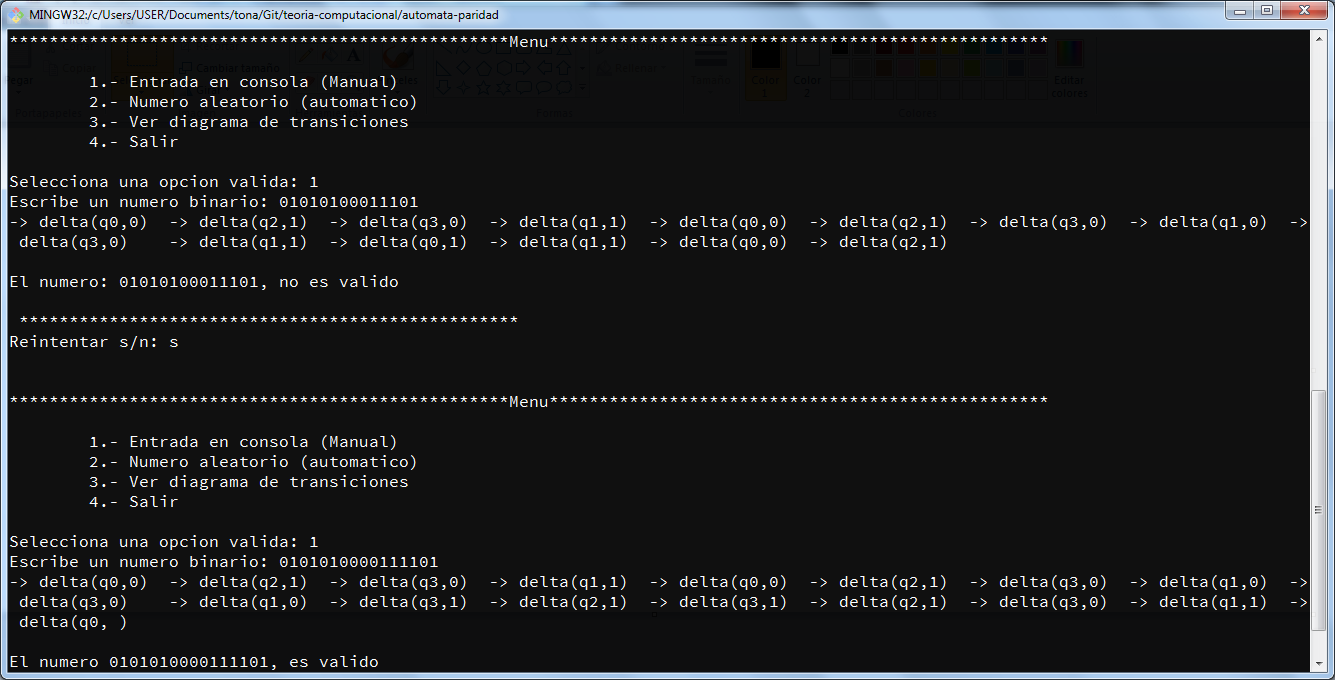
\includegraphics[width=\linewidth, height=8cm]{img/manual-paridad.png}
			\caption{Historia del autómata}
			\label{fig:paridad2}
		\end{center}
	\end{figure}
	{\large Modo automático.}
	\begin{figure}[H]
		\begin{center}
			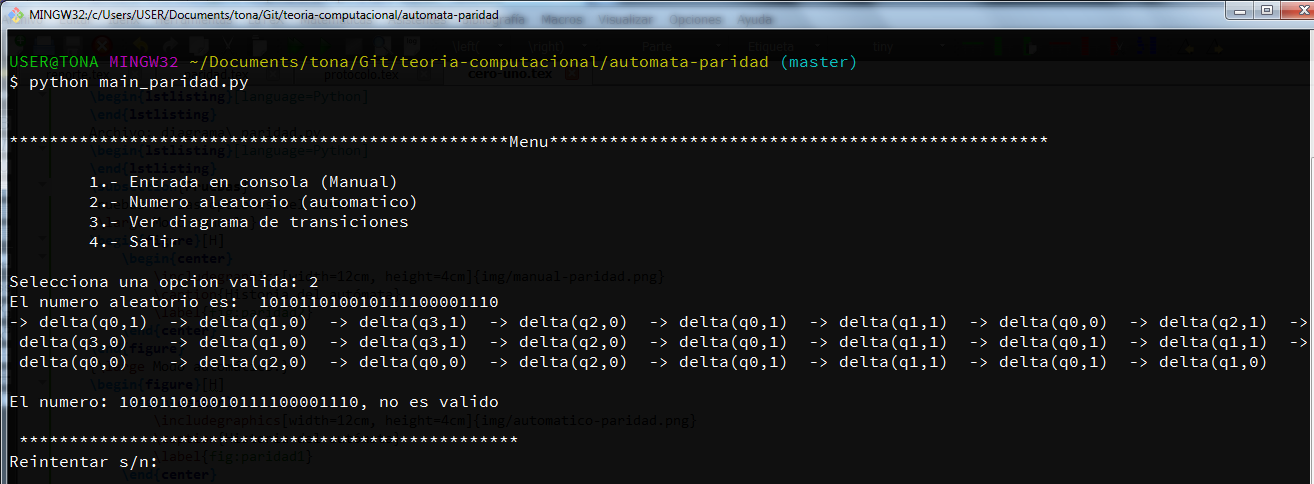
\includegraphics[width=\linewidth, height=8cm]{img/automatico-paridad.png}
			\caption{Historia del autómata}
			\label{fig:paridad1}
		\end{center}
	\end{figure}
	{\large Diagrama.}
	\begin{figure}[H]
		\begin{center}
			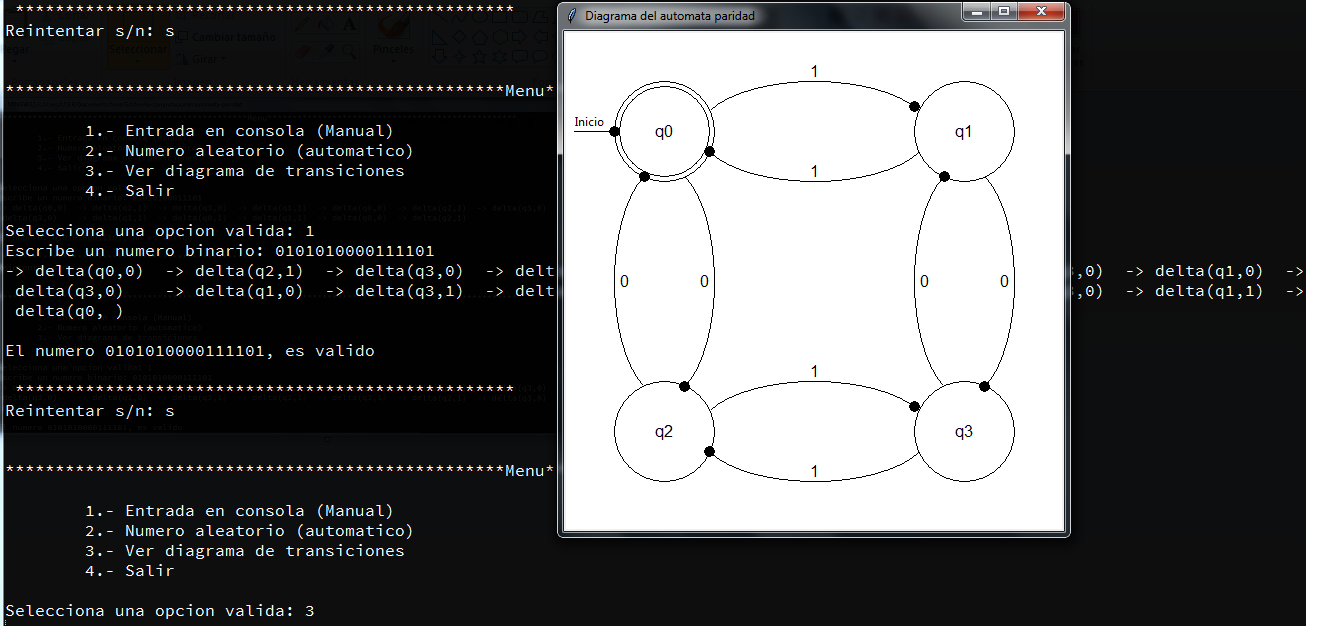
\includegraphics[width=\linewidth, height=8cm]{img/diagrama-paridad.png}
			\caption{Diagrama de transiciones del autómata}
			\label{fig:paridad3}
		\end{center}
	\end{figure}